% author: 'Marie Lohbeck'
% copyright: 'Copyright 2018, Advanced UniByte GmbH'
%
% license notice:
%
% This file is part of PicDat.
% PicDat is free software: you can redistribute it and/or modify it under the terms of the GNU
% General Public (at your option) any later version.
%
% PicDat is distributed in the hope that it will be useful, but WITHOUT ANY WARRANTY; without
% even the implied warranty of MERCHANTABILITY or FITNESS FOR A PARTICULAR PURPOSE. See the GNU
% General Public License for more details.
%
% You should have received a copy of the GNU General Public License along with PicDat. If not,
% see <http://www.gnu.org/licenses/>.

\documentclass[8pt]{beamer}
\mode<presentation>
{
  \setbeamercovered{transparent}
  \setbeamertemplate{navigation symbols}{} % no navigation bar
}
\usepackage[T1]{fontenc}
\usepackage[utf8]{inputenc}
\usepackage{lmodern}
\usepackage{listings}
\usepackage{color}
\usepackage{hyperref}

\definecolor{grey}{rgb}{0.8, 0.8, 0.8}
\definecolor{darkblue}{rgb}{0.15, 0.38, 0.61}
\setbeamercolor{frametitle}{fg=darkblue}

\lstset{frame=tb,
  aboveskip=1mm,
  belowskip=1mm,
  showstringspaces=false,
  columns=flexible,
  basicstyle={\tiny\ttfamily\color{darkblue}},
  breaklines=true,
  breakatwhitespace=true,
  rulecolor=\color{grey}
}
\begin{document}

\begin{frame}
\frametitle{PicDat -- Instruction}
\begin{figure}
	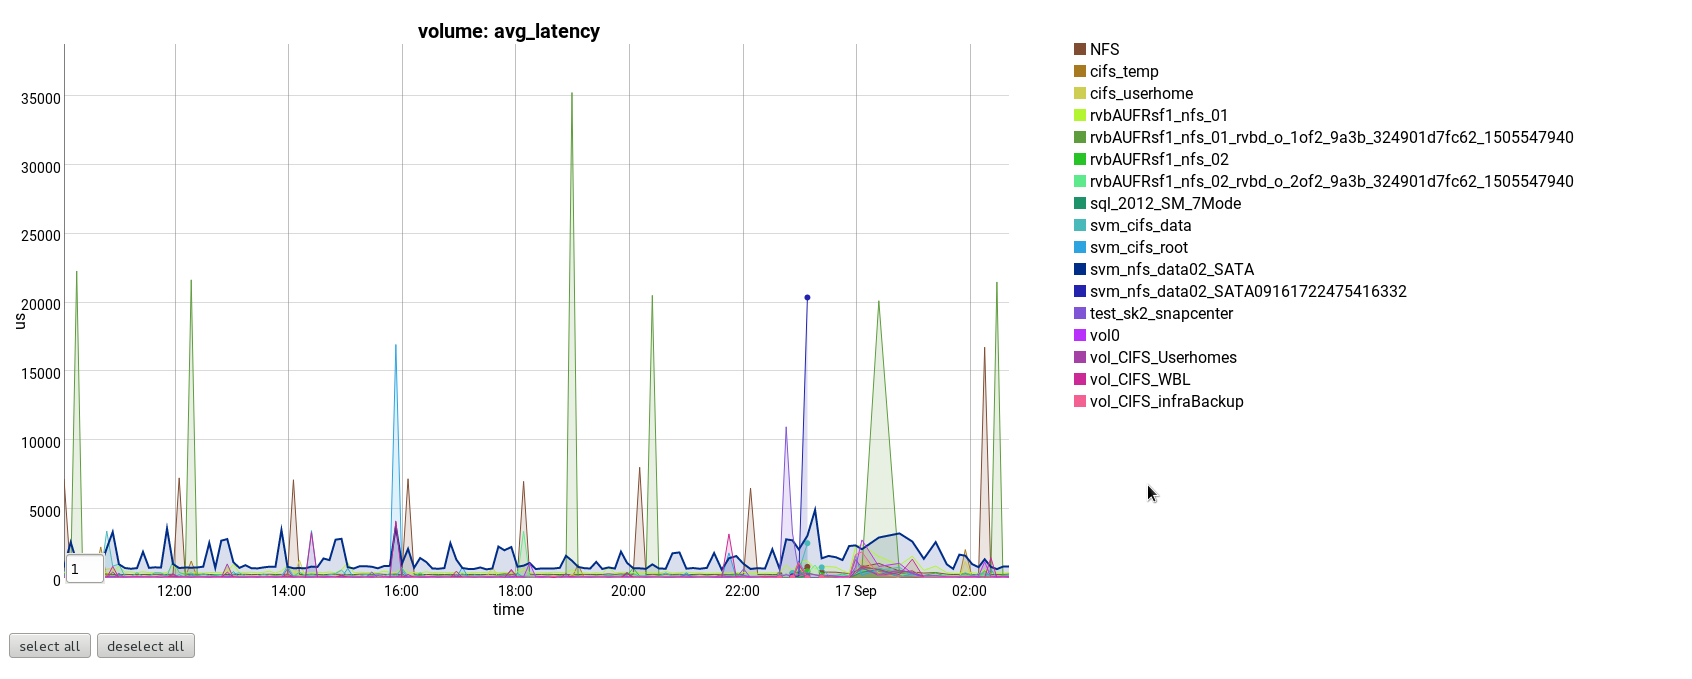
\includegraphics[width=\textwidth]{../images/PicDat_normal.png}
\end{figure}
The aim of PicDat is to provide better insight to performance data from NetApp controllers. The command line tool is able to visualize data from both PerfStat output and ASUP files.

PicDat selects some counters of such files which are typically sufficient for the analysis and writes them to several csv tables. Then it generates a HTML file using a JavaScript library called dygraphs to visualize those tables. Open the HTML in a browser to get your performance charts.
\end{frame}

\begin{frame}
\frametitle{Table of contents}

\tableofcontents
\end{frame}

\section{Running PicDat}
\begin{frame}
\frametitle{Running PicDat}
You can run PicDat without any parameters. After you startet it, it'll ask you for some performance input. Additionally, PicDat will ask you to enter a directory for its results. Be aware, that content might become overwritten if this directory is not empty. After this, PicDat will start working. 
\bigskip

Alternatively, you can pass input and output specifications as command line parameters. Therefore, use the options \textcolor{darkblue}{\texttt{-\,-inputfile}} and \textcolor{darkblue}{\texttt{-\,-outputdir}} or \textcolor{darkblue}{\texttt{-i}} and \textcolor{darkblue}{\texttt{-o}} respectively.
\smallskip
\end{frame}

\section{Run example}
\begin{frame}[fragile]
\frametitle{Run example}
This is how a run could look like on your command line:
\smallskip

\begin{lstlisting}
python picdat.py -i"</path/to/input>" -o"</path/to/output>" 
2018-03-09 12:00:35,195 INFO: inputfile: </path/to/input>, outputdir: </path/to/output>
2018-03-09 12:00:35,196 INFO: Prepare directory...
2018-03-09 12:00:35,202 INFO: Running PicDat in PerfStat mode
2018-03-09 12:00:35,202 INFO: Did not find a console.log file to extract perfstat's cluster and node name.
2018-03-09 12:00:35,202 INFO: Read data...
2018-03-09 12:00:37,796 INFO: Planned number of iterations was executed correctly.
2018-03-09 12:00:37,798 INFO: Create csv tables...
2018-03-09 12:00:37,799 INFO: Wrote chart values into /path/to/output/tables/aggregate_total_transfers_chart_values.csv
2018-03-09 12:00:37,799 INFO: Wrote chart values into /path/to/output/tables/processor_processor_busy_chart_values.csv
2018-03-09 12:00:37,799 INFO: Wrote chart values into /path/to/output/tables/volume_read_ops_chart_values.csv
2018-03-09 12:00:37,801 INFO: Wrote chart values into /path/to/output/tables/volume_write_ops_chart_values.csv
2018-03-09 12:00:37,801 INFO: Wrote chart values into /path/to/output/tables/volume_other_ops_chart_values.csv
2018-03-09 12:00:37,801 INFO: Wrote chart values into /path/to/output/tables/volume_total_ops_chart_values.csv
2018-03-09 12:00:37,802 INFO: Wrote chart values into /path/to/output/tables/volume_avg_latency_chart_values.csv
2018-03-09 12:00:37,802 INFO: Wrote chart values into /path/to/output/tables/volume_read_data_chart_values.csv
2018-03-09 12:00:37,802 INFO: Wrote chart values into /path/to/output/tables/volume_write_data_chart_values.csv
2018-03-09 12:00:37,807 INFO: Wrote chart values into /path/to/output/tables/sysstat_1sec_percent_chart_values.csv
2018-03-09 12:00:37,819 INFO: Wrote chart values into /path/to/output/tables/sysstat_1sec_MBs_chart_values.csv
2018-03-09 12:00:37,828 INFO: Wrote chart values into /path/to/output/tables/sysstat_1sec_IOPS_chart_values.csv
2018-03-09 12:00:37,830 INFO: Wrote chart values into /path/to/output/tables/statit_disk_statistics_chart_values.csv
2018-03-09 12:00:37,831 INFO: Create html file...
2018-03-09 12:00:37,833 INFO: Generated html file at /path/to/output/charts.html
2018-03-09 12:00:37,843 INFO: Done. You will find charts under: </path/to/output>
\end{lstlisting}
\smallskip

General usage: 
\smallskip
\begin{lstlisting}
picdat [--help] [--sortbyname] [--inputfile "input"] [--outputdir "output"] [--debug "level"] [--logfile]
\end{lstlisting}
\end{frame}

\section{Command line options}
\begin{frame}[label=options]
\frametitle{Command line options}
Additional to \textcolor{darkblue}{\texttt{-\,-inputfile}} and \textcolor{darkblue}{\texttt{-\,-outputdir}}, there are following command line options available:
\bigskip

The \textcolor{darkblue}{\texttt{-\,-debug}} or \textcolor{darkblue}{\texttt{-d}} option specifies the filtering level for command line output. Pass it together with a string out of those: \texttt{debug, info, warning, error, critical}. Default is \texttt{info}.
\bigskip

If you wand to redirect the command line output into a log file for further analysis, use the flag \textcolor{darkblue}{\texttt{-\,-logfile}} or \textcolor{darkblue}{\texttt{-l}}. This will create a picdat.log file inside your output directory.
\bigskip

By default, PicDat sorts the most data series by relevance. This means, the graph with the highest sum of values will be displayed at the top of a chart's legend. If you rather wants them to be sorted alphanumeric, use the flag \textcolor{darkblue}{\texttt{-\,-sortbyname}} or \textcolor{darkblue}{\texttt{-s}}.
\bigskip

PicDat needs the dygraph library as well as the csv data files to show charts in a browser. But some browsers like Google Chrome or Edge refuse to load additional local files for security reasons. Hence, PicDat charts just stay empty. To avoid this, use option \textcolor{darkblue}{\texttt{-\,-compact}} or \textcolor{darkblue}{\texttt{-c}}. This option packs all code and data into the HTML file. The dygraph.js and dygraph.css files don't get copied to your result directory anymore. The csv data files still get created, but the charts.html file don't reference them. So, the result is even more portable, because you can copy the single HTML file without caring for any dependencies.
\bigskip

To get an overview about all command line option, try option \textcolor{darkblue}{\texttt{-\,-help}} or \textcolor{darkblue}{\texttt{-h}}.
\end{frame}

\section{Input format}
\subsection{PerfStat mode}
\begin{frame}
\frametitle{Input format -- PerfStat mode}
As mentioned, PicDat can handle different kinds of performance data.
\bigskip

If you want to visualize \textcolor{darkblue}{\textbf{PerfStat data}}, you have following options: Either you can pass single PerfStat data files (they have to end with \textbf{.data} or \textbf{.out}) or you can pass a \textbf{directory}, containing such files. Furthermore, you can pass a \textbf{.zip} file containing PerfStat output. If you transmit a single file, be aware, that some meta data which are usually packed together with PerfStats, will not be readable. If you transmit several PerfStats (within a directory or zip), PicDat will generate \textbf{one HTML} with charts \textbf{for each PerfStat}. 
\end{frame}

\subsection{ASUP mode}

\begin{frame}
\frametitle{Input format -- ASUP mode}
How an \textcolor{darkblue}{\textbf{ASUP}} looks like depends on the os version of your NetApp machine. PicDat currently supports \textbf{ASUPs of Ontap 9}. Among the minor versions of Ontap 9, there are two different data types for performance data in the ASUPs -- xml and ccma. XML is human readable and can be processed by PicDat directly. Ccma files in contrast must be preprocessed by a tool called \hyperref[trafero]{Trafero} first.
\bigskip

In the first place, this means for you to check which kind of data your ASUP contains. From Ontap versions up to 9.2, automatic ASUPs get createt in XML format. For Ontap 9.2 and higher, automatic ASUPs will be in ccma format. But if you trigger an ASUP manually, so that it appears under the 'On Demand History', ccma format will be present even for previous versions. How you can convert ccma ASUPs into readable JSON, which is again processable by PicDat, is described in section \hyperref[trafero]{\underline{Use Trafero}}.

To deal with the different kinds of input, PicDat divides the ASUP mode into two sub modes: \textbf{ASUP XML mode} and \textbf{ASUP JSON mode}. The mode's input formats are described precisely on the following slides.
\end{frame}

\subsubsection{XML}

\begin{frame}
\frametitle{Input format -- ASUP XML mode}
\textcolor{darkblue}{\textbf{ASUP XML}} data is available in automatically generated ASUPs for Ontap 9.0 or Ontap 9.1. The whole ASUP usually is a tar archive with file extension \textbf{.tgz}. You can pass it as input in a whole. It is also possible to transmit the unpacked tar, i.e. a \textbf{directory}. There is nothing as a single file transmission as in Perfstat mode, because PicDat needs at least two files from the ASUP, a CM-STATS-HOURLY-INFO.XML and a CM-STATS-HOURLY-DATA.XML file for its analysis.
\bigskip

Working with ASUPs, it might be useful to visualize data for several consecutive ASUP files together. To do so, just pack \textbf{several ASUP .tgz archives into one directory} and pass the directory to PicDat. Therefore, the alphabetical order of the archive names should go with the chronological order. PicDat will stick the results for the different data files together. This means, different from visualizing PerfStats, only \textbf{one HTML for all data} will be generated. So don't mess around and pack ASUP files into one folder, which don't belong together! Don't mix nodes.
\end{frame}

\subsubsection{JSON}

\begin{frame}
\frametitle{Input format -- ASUP JSON mode}
From os version ontap 9.2, ASUPs don't provide permormance data in XML format anymore. Instead, there are files with a ccma file extension. This applies also to 'on Demand' ASUPs. Luckily, you can use the tool \hyperref[trafero]{\underline{Trafero}} to transform them into JSON.
\bigskip

For JSON data, PicDat provides the \textcolor{darkblue}{\textbf{ASUP JSON mode}}. To use this mode, give PicDat either a single \textbf{.json} file as input or a \textbf{directory with JSON files inside}. If you give several JSONs, make sure they all belong to the same cluster and node! Besides this, it doesn't matter a lot how the information is splitted over the several files. As each JSON object contains all necessary information about a value, PicDat will read one after another without caring about their order.
\end{frame}

\subsubsection{Comment about HDF5}

\begin{frame}
\frametitle{Comment about HDF5}
During conversion of ccma files with Trafero, an additional file with performance data gets created: A HDF5 file. PicDat tried to deal with this file in the first place. Therefore, there was the additional mode \textcolor{darkblue}{\textbf{ASUP HDF5}}. But the HDF5 files do not contain all necessary information, so PicDat now uses Trafero's JSON output instead.
\bigskip

So, the ASUP HDF5 mode is deprecated now. But, technically, it still works, so it is mentioned here. To use it, give PicDat a single \textbf{.h5} file as input; something like directory or archive transmission is not possible. PicDat will create \textbf{one HTML} per input file. 
\end{frame}

\section{Use Trafero}

\begin{frame}[fragile, label=trafero]
\frametitle{Use Trafero}
If you have an ASUP from a Netapp machine with os version \textbf{Ontap 9.2 or later}, or an \textbf{onDemand} ASUP, you need to preprocess it with a Netapp tool called Trafero before PicDat understands it.

Trafero is embedded into a bigger tool called 'NetApp Active IQ PAS' using Docker. Its documentation can be find here: \url{http://aiqpas-metadata.s3-website-us-east-1.amazonaws.com/}

You will need a NetApp account to get it.
\bigskip

Assuming that you have access to a running docker container with a working Trafero installation, you can perform the conversion with a script called \textcolor{darkblue}{\textbf{convert\_ccma\_to\_json.py}}. You'll find it under picdatscripts.
\bigskip

Call the script for example like:

\begin{lstlisting}
python convert_ccma_to_json.py -i"</path/to/your/ASUP_with_ccma.tgz" -o"</favorite/output/directory>"
\end{lstlisting}

This will copy and extract your ASUP to the Trafero container, ingest the ASUP into the Trafero database, Request the values of this ASUP in JSON format, writes the values in several .json file into your output directory, deletes the ASUP from the Trafero database, and finally removes the extracted ASUP files from the Trafero container. All command line options can be shown with \textcolor{darkblue}{\texttt{-\,-help}}.
\bigskip

Be aware that you need the correct \textcolor{darkblue}{\textbf{config.yml}} file in the same location as the script while running. This file specifies, how the Trafero container can be accessed and which objects and counters will be collected while conversion. 
\end{frame}

\section{Interactive charts}
\subsection{Interactive charts -- legend}
\begin{frame}
\frametitle{Interactive charts -- legend}
The Job of PicDat is to pick and visualize some of the various information given with the input. The charts.html files contain multiple labeled charts offering some interaction. They are arranged in several Tabs.

\begin{figure}
	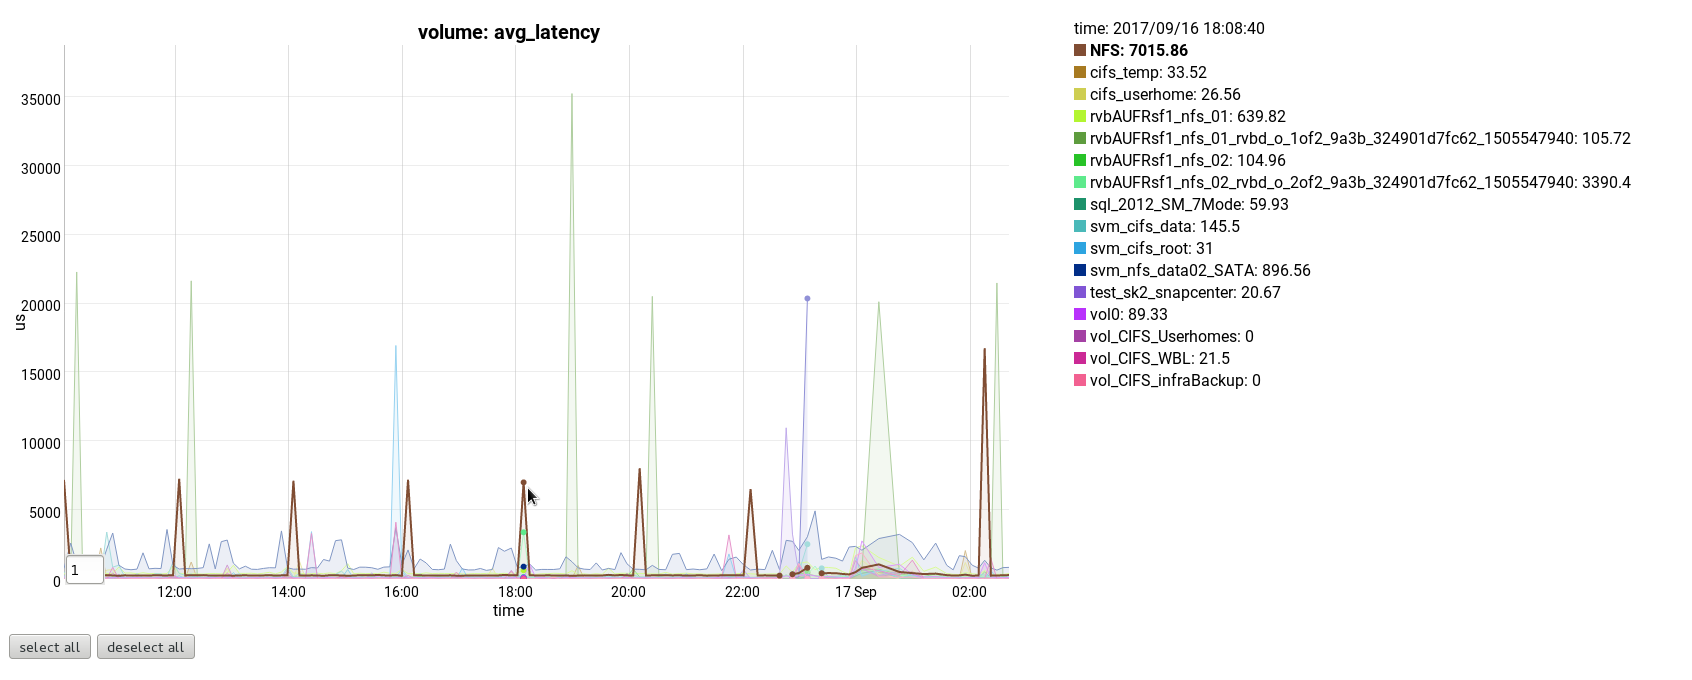
\includegraphics[width=\textwidth]{../images/PicDat_highlight2.png}
\end{figure}

Mouse-over the charts to display the values in the legend. You'll notice as well, that the graph, your cursor is next to, will be highlighted. The corresponding entry in the legend will be highlighted similtaneously.
\end{frame}

\begin{frame}
\frametitle{Interactive charts -- legend} 
\begin{figure}
	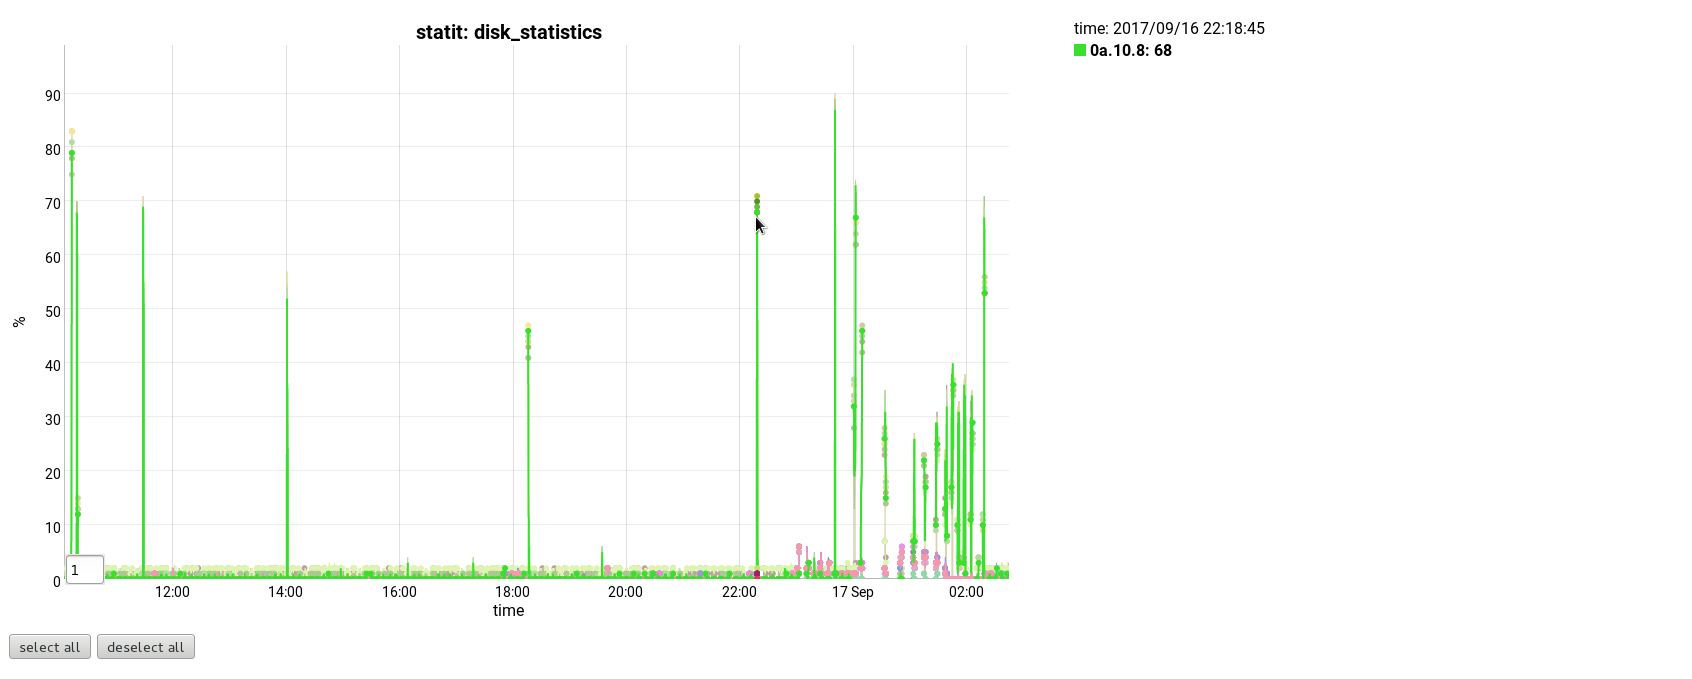
\includegraphics[width=\textwidth]{../images/PicDat_singleValue.png}
\end{figure}

If there are so many graphs in one chart that the legend can't display them all without a scroll bar, the legend will change to display only one value at once as soon as your mouse enters the chart.
\end{frame}

\subsection{Interactive charts -- zoom}
\begin{frame}
\frametitle{Interactive charts -- zoom} 
\begin{figure}
	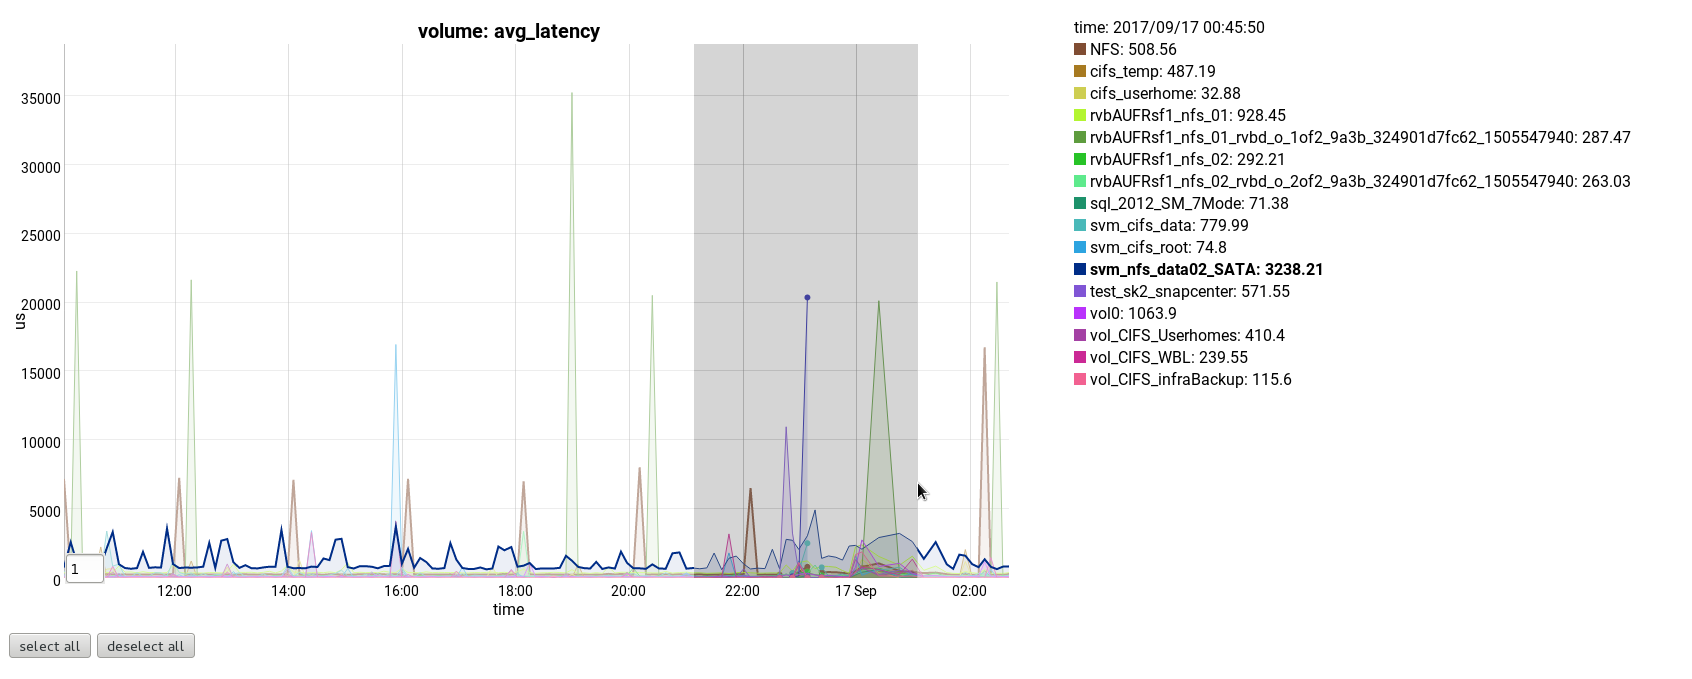
\includegraphics[width=\textwidth]{../images/PicDat_zoomVertical.png}
\end{figure}

To zoom inside the charts, just click and drag them in x or y direction. Once zoomed in, you can also change the displayed range by holding shift an click and drag again. To go back into original view, just double-click the chart.
\end{frame}

\subsection{Interactive charts -- select and deselect}
\begin{frame}
\frametitle{Interactive charts -- select and deselect} 
\begin{figure}
	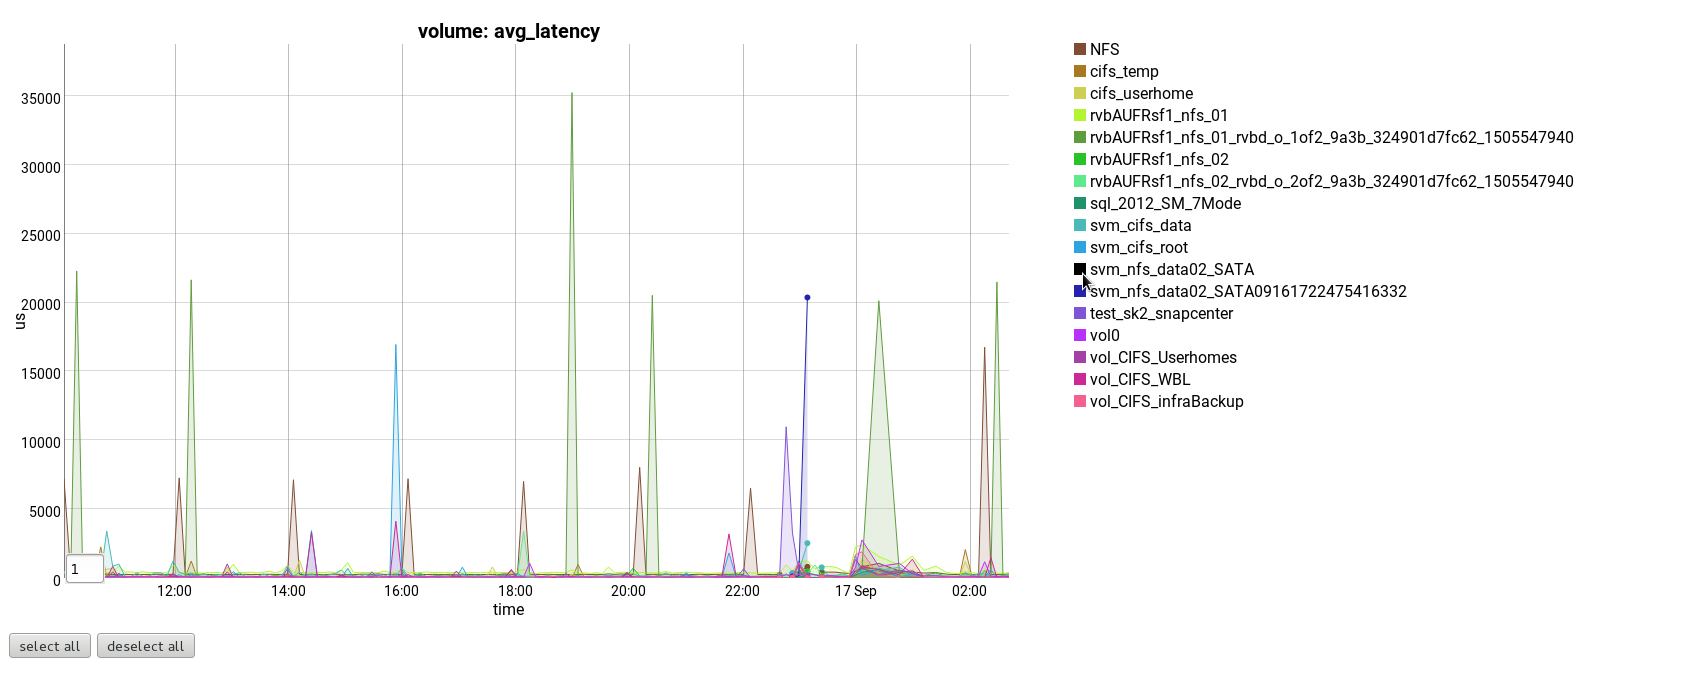
\includegraphics[width=\textwidth]{../images/PicDat_deselect.png}
\end{figure}

You might wish to take some graph lines out of view. Therefore, click one of the colored boxes inside the legend. It'll turn to black and the corresponding graph will disappear from sight. Click it again and the graph will come back. To select or deselect all lines at once, use the buttons beneath the chart.
Note, that disabled graphs disappear from the legend whereas your cursor is on the chart. Entries, belonging to graphs with a gap at the place your cursor recently is, will disappear as well. So don't be confused if the legend will bounce a bit as you move your mouse.
\end{frame}

\subsection{Interactive charts -- rolling average}
\begin{frame}
\frametitle{Interactive charts -- rolling average} 
\begin{figure}
	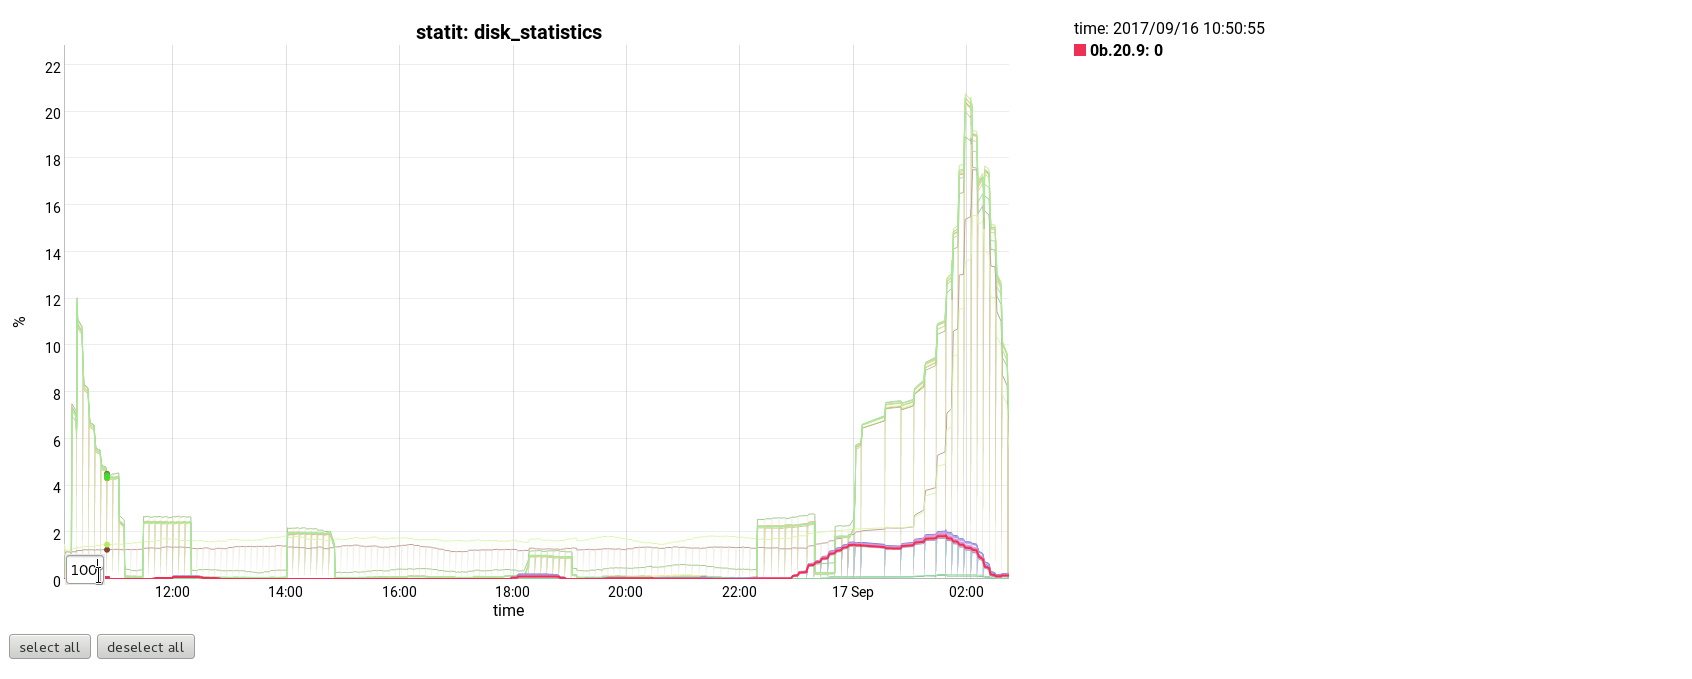
\includegraphics[width=\textwidth]{../images/PicDat_roller.png}
\end{figure}

If your values are very close and unsteady, you might get a better overview using a rolling average. Therefore, type a natural number into the small textfield appearing at the lower left corner of most charts. After hitting 'enter', the data will get averaged over this number of measuring points.
\end{frame}

\section{Can't see any graphs?}
\begin{frame}
\frametitle{Can't see any graphs?}
If PicDat seems to ran correctly, but all charts inside the charts.html are empty, see whether one of the following applies:
\bigskip

If you are running the charts.html from your file system, the browsers Chrome and Internet Explorer/Edge will block external files for security reasons. So, the dygraph.js don't get loaded. As workaround, PicDat provides the command line option \textcolor{darkblue}{\texttt{-\,-compact}}, which packs all the output into one file (See \hyperref[options]{\underline{Command line options}}). Alternatively, use Firefox instead or try to change security settings.
\bigskip

If this is not the problem, make sure that dygraphs is available at all. As long as you haven't used option \textcolor{darkblue}{\texttt{-\,-compact}}, a folder called 'dygraphs', containing the dygraph.js and dygraph.css, must be in the same location as your charts.html file. Of course, a folder called 'tables' which contains all chart data within csv tables must be available too.
\end{frame}

\end{document}
